\begin{figure}[H]
	\centering
	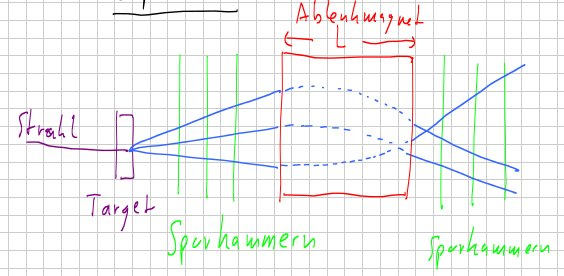
\includegraphics[width=0.5\textwidth]{fixed1.jpg}
	\caption{	 ???}
	\label{fixed1}
\end{figure}

\begin{figure}[H]
	\centering
	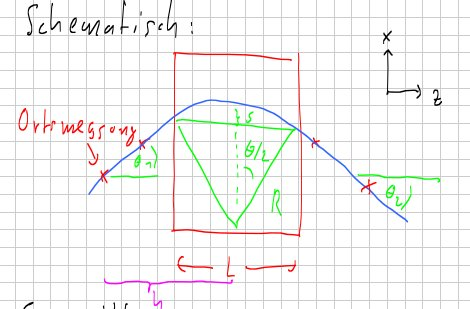
\includegraphics[width=0.5\textwidth]{fixed2.jpg}
	\caption{	 ???}
	\label{fixed2}
\end{figure}

Aus den obigen Zeichnungen lässt sich ableiten: 

\[ 2\cdot \text{sin}\,\frac{\Theta}{2} = \frac{L}{R} = -e\cdot B_y\cdot \frac{L}{p} \]

Der Impuls $p_x$ wird also um 

\[ \Delta p_x = p\cdot \text{sin}\,\Theta \]

geändert, sodass für kleine Winkelablenkungen $\Theta$ gilt

\[ \Delta p_x \approx -e\cdot B_y\cdot L = -e \int B_y \mathrm{d}z.\]

Ein Feldintegral von $\int B_y \mathrm{d}z$ von $1\,$Tm beispielsweise ergibt eine Impulsänderung
von $\Delta p_x \approx 0{,}3\,$GeV/c.
\\
Der Impuls des Teilchens folgt dann aus der Winkeländerung $\Theta$ und dem Feldintegral $\int B
\mathrm{d}z$:

\begin{align*}
\text{sin}\,\Theta &= \text{sin}\,(\Theta_2-\Theta_1) \\
&= \text{sin}\,\Theta_2\text{cos}\,\Theta_1-\text{sin}\,\Theta_1\text{cos}\,\Theta_2 \\
&\approx \text{sin}\,\Theta_2-\text{sin}\,\Theta_1
\end{align*}


Wegen

\[p=e\cdot B_y \frac{L}{2\cdot \text{sin}\,\frac{\Theta}{2}} \approx e\cdot B_y \frac{L}{\Theta} \] 

gilt

\[ \left| \frac{\mathrm{d}p}{\mathrm{d}\Theta} \right| =e\cdot B_y\cdot L \cdot \frac{1}{\Theta^2} =
\frac{p}{\Theta} \]

und damit für die Impulsauflösung

\[ \frac{\sigma(p)}{p}  = \frac{\sigma(\Theta)}{\Theta}. \]

Mit mindestens vier Ortsmessungen mit Hebelarm $h$ ist $\Theta=\frac{x}{h}$, also

\[\sigma^2(\Theta) \approx \sum_{i=1}^4 \sigma_i^2(x) \approx 4\cdot \sigma^2(x)  \]
\[\Rightarrow~~~ \sigma(\Theta) \sim 2\cdot\sigma(x). \]

Damit ist die Impulsmessgenauigkeit

\[ \frac{\sigma(p)}{p} = \frac{2\cdot\sigma(x)/h}{e\cdot B_y\cdot L}\cdot p =
\frac{2\cdot\sigma(x)}{h}\cdot \frac{p}{\Delta p_x} \]

d.h. die Impulsauflösung ist proportional zum Impuls $p$.
\\
Zum Beitrag aus der Ortsmessung kommt noch die Vielfachstreuung hinzu:

\[\Delta p_x^{\text{VS}} = p\cdot \text{sin}\,\Theta^{\text{VS}}_{\text{rms}} \approx p \cdot
\Theta^{\text{VS}}_{\text{rms}} \]
\[ \Rightarrow~~~ \Delta p_x^{\text{VS}} \approx \frac{19{,}2\,\text{MeV/c}}{\sqrt{2}}\cdot
\sqrt{\frac{L}{x_0}} \]

d.h. $\Delta p_x^{\text{VS}}$ ist unabhängig von $p$. Der Gesamtfehler ist dann die quadratische
Summe, also

\[ \frac{\sigma(p)}{p} = \frac{\sigma^{\text{out???}}(p)}{p} \oplus
\frac{\sigma^{\text{up???}}(p)}{p} = \sqrt{a^2p^2+b^2}\]

wobei $a\oplus b = \sqrt{a^2+b^2}$. Der Gesamtfehler wächst also mit zunehmendem Impuls an.

\begin{figure}[H]
	\centering
	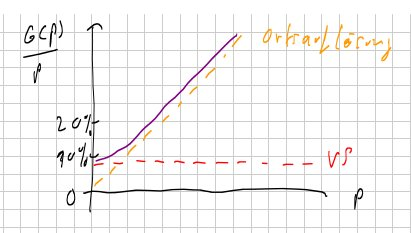
\includegraphics[width=0.5\textwidth]{fixed3.jpg}
	\caption{	 ???}
	\label{fixed3}
\end{figure}